\section{فرضیات مدل‌سازی}\label{sec_modelassum}
شماتیک استند چهارپره در شكل \ref{QuadAssum} نشان داده شده‌است.
% به ‌منظور استخراج معادلات حاکم بر سیستم، 
%فرض می‌شود که چهارپره صلب و متقارن است. همچنین ماتریس گشتاور اینرسی چهارپره به‌صورت قطری درنظر گرفته می‌شود. مرکز جرم سازه چهارپره روی نقطه $B$ و مرکز ثقل هر یک از پره‌ها به همراه قسمت دوار موتور روی نقاط 
%$B_1$
%تا
%$B_4$
%است. مبدأ دستگاه مختصات بدنی روی محل تقاطع بازوهای چهارپره یعنی نقطه 
%$B$
%در نظر گرفته شده است. از آنجایی ‌که مرکز ثقل پره‌ها بالاتر از مرکز ثقل سازه چهارپره است، مرکز ثقل کلی چهارپره جایی بین مرکز ثقل موتورها و سازه، یعنی نقطه‌ی 
%$C$
%می‌گیرد. همچنین قابل ذکر است که نقطه‌ی
%$D$
%محل اتصال کلی استند چهارپره است. جهت مثبت محور 
%$X^B$
%و
%$Y^B$
%دستگاه مختصات بدنی به ترتیب در راستای بازوی مربوط به موتور 1 و 4 فرض می‌شود. همچنین جهت مثبت محور
%$Z^B$
%با توجه به قانون دست راست حاصل می‌شود.
\begin{figure}[H]
	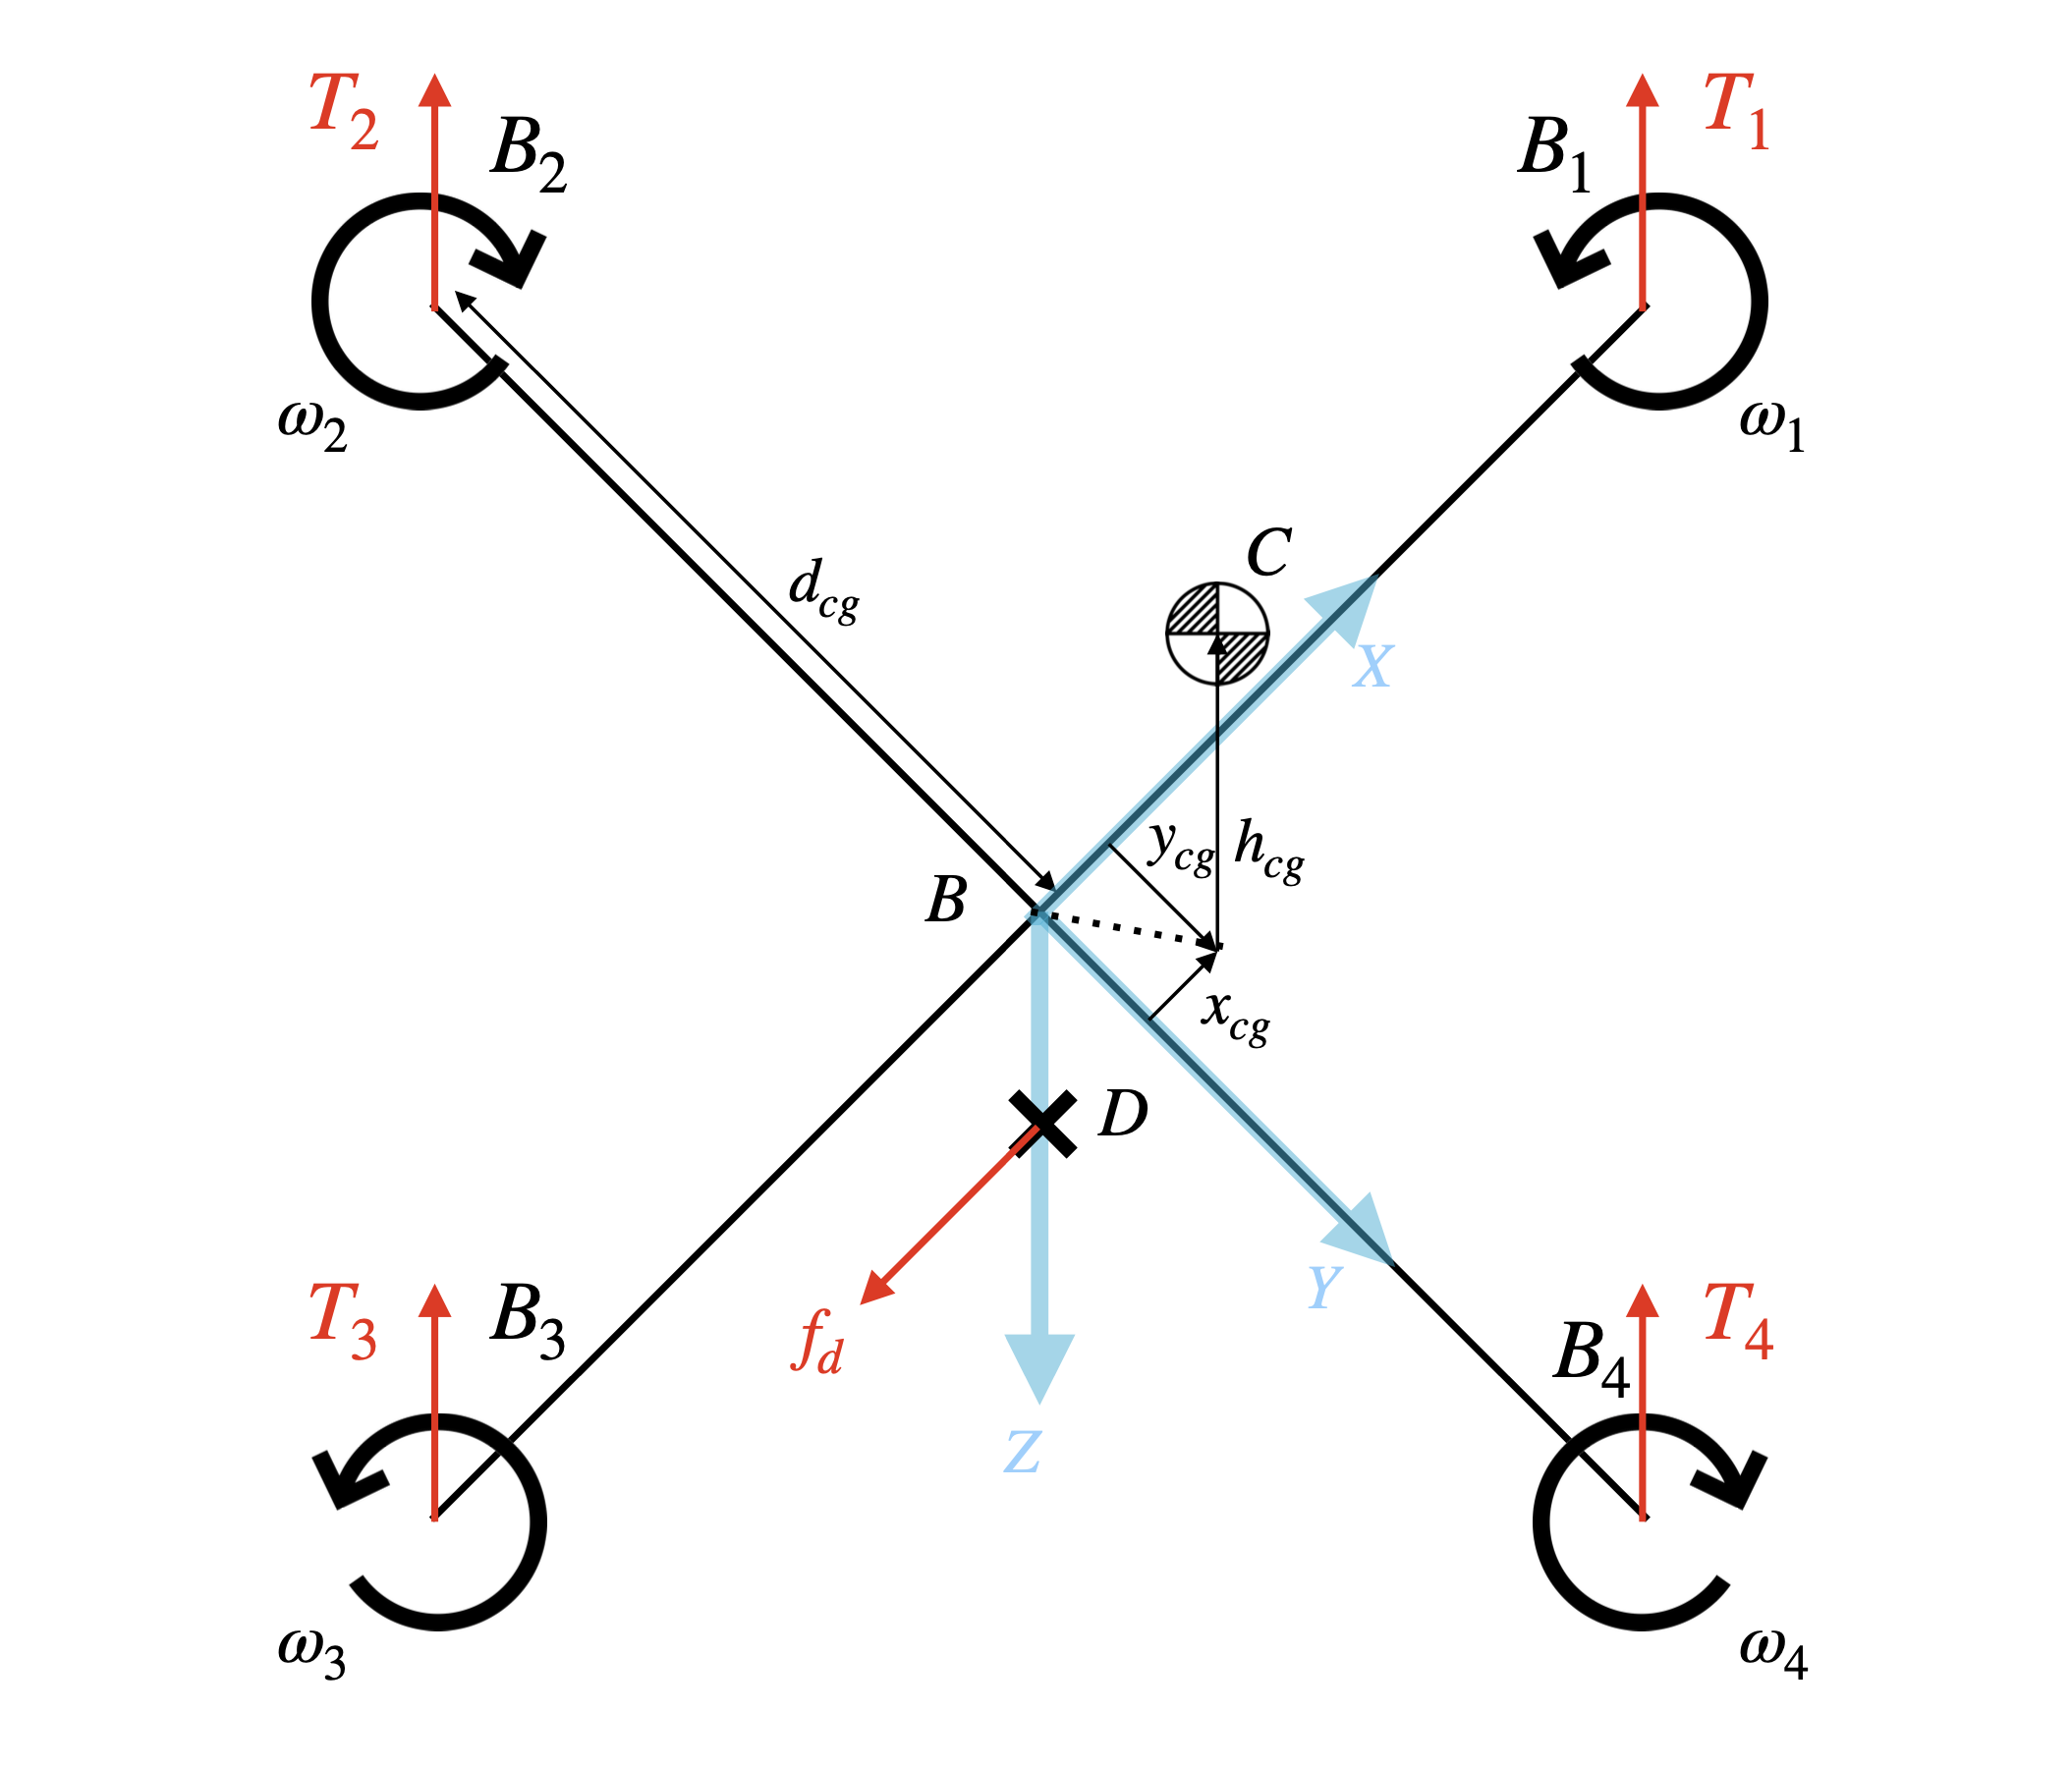
\includegraphics[width=12cm]{../Figures/Forces/StandAssumations.png}
	\centering
	\caption{شماتیک استند چهارپره}
	\label{QuadAssum}
\end{figure}